\usetikzlibrary{matrix, calc}

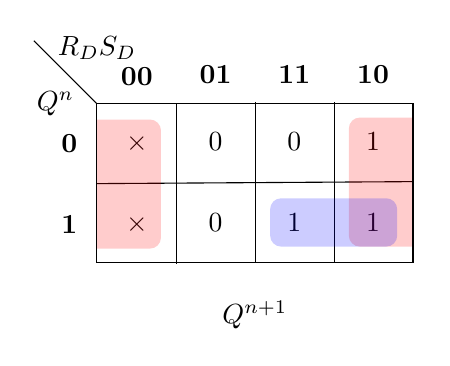
\begin{tikzpicture}

    % Define the Karnaugh map matrix
    \matrix (km) [
        matrix of math nodes,
        nodes in empty cells,
        nodes={minimum size=1cm}
    ]{
        \times & 0 & 0 & 1 \\
        \times & 0 & 1 & 1 \\
    };

    Draw vertical lines
    \foreach \col in {1,2,3}{
            \draw (km-1-\col.north east) -- (km-2-\col.south east);
        }

    Draw horizontal line
    \draw (km-1-1.south west) -- (km-1-4.south east);

    Draw diagonal line
    \draw (km-1-1.north west) -- ++(-0.8, 0.8);

    Add labels
    \node[yshift=10, font=\bfseries] at (km-1-1.north) {00};
    \node[yshift=10, font=\bfseries] at (km-1-2.north) {01};
    \node[yshift=10, font=\bfseries] at (km-1-3.north) {11};
    \node[yshift=10, font=\bfseries] at (km-1-4.north) {10};
    \node[xshift=-10, font=\bfseries] at (km-1-1.west) {0};
    \node[xshift=-10, font=\bfseries] at (km-2-1.west) {1};
    \node[yshift=20] at (km-1-1.north west) {$R_DS_D$};
    \node[xshift=-15] at (km-1-1.north west) {$Q^n$};
    \node[yshift=-15] at (km.south) {$Q^{n+1}$};

    % Draw Marked
    \fill[rounded corners, red, opacity=0.2]
        ($(km-1-4.north east) + (0, -0.2)$)
        -- ($(km-1-4.north west) + (0.2, -0.2)$)
        -- ($(km-2-4.south west) + (0.2, 0.2)$)
        -- ($(km-2-4.south east) + (0, 0.2)$);
    \fill[rounded corners, red, opacity=0.2]
        ($(km-1-1.north west) + (0, -0.2)$)
        -- ($(km-1-1.north east) + (-0.2, -0.2)$)
        -- ($(km-2-1.south east) + (-0.2, 0.2)$)
        -- ($(km-2-1.south west) + (0, 0.2)$);
    \fill[rounded corners, blue, opacity=0.2]
        ($(km-2-3.north west) + (0.2, -0.2)$)
        -- ($(km-2-4.north east) + (-0.2, -0.2)$)
        -- ($(km-2-4.south east) + (-0.2, 0.2)$)
        -- ($(km-2-3.south west) + (0.2, 0.2)$)
        -- cycle;

    Draw a rectangle around the matrix
    \draw (km-1-1.north west) rectangle (km-2-4.south east) {};

\end{tikzpicture}